\documentclass[conference]{IEEEtran}

\usepackage{multirow}
\usepackage{subfigure}
\usepackage{graphicx}
\usepackage{graphics}
\usepackage{rotating}
\usepackage{verbatim}
\usepackage{float}
\usepackage{lipsum}
\usepackage{url}
\usepackage{wrapfig}
\usepackage{tabularx}
\usepackage{amsmath}
\usepackage{listings}
\usepackage{color}
\definecolor{javared}{rgb}{0.6,0,0} % for strings
\definecolor{javagreen}{rgb}{0.25,0.5,0.35} % comments
\definecolor{javapurple}{rgb}{0.5,0,0.35} % keywords
\definecolor{javadocblue}{rgb}{0.25,0.35,0.75} % javadoc
 
\lstset{language=Java,
basicstyle=\ttfamily,
keywordstyle=\color{javapurple}\bfseries,
stringstyle=\color{javared},
commentstyle=\color{javagreen},
morecomment=[s][\color{javadocblue}]{/**}{*/},
%numbers=left,
numberstyle=\tiny\color{black},
stepnumber=2,
numbersep=10pt,
tabsize=4,
showspaces=false,
showstringspaces=false}

\newcommand\blfootnote[1]{%
  \begingroup
  \renewcommand\thefootnote{}\footnote{#1}%
  \addtocounter{footnote}{-1}%
  \endgroup
}
%\restylefloat{table}

%\ifCLASSINFOpdf
%\else
%\fi
%\hyphenation{op-tical net-works semi-conduc-tor}
\begin{document}
\title{ADFD+: An Automatic Tool for Finding and Presenting Failure domains}
\author{Mian Asbat Ahmad and Manuel Oriol}
%\author{\IEEEauthorblockN{Mian Asbat Ahmad}
%\IEEEauthorblockA{Department of Computer Science\\
%University of York\\
%York, United Kingdom\\
%Email: mian.ahmad@york.ac.uk}
%\and
%\author{Manuel Oriol}
%\IEEEauthorblockN{Manuel Oriol}
%Department of Computer Science\\
%University of York\\
%York, United Kingdom\\
%Email: manuel.oriol@york.ac.uk
%}
\maketitle
\vspace*{0\baselineskip}
\IEEEtitleabstractindextext{
\begin{abstract}
%This paper verifies the accuracy of invariants generated automatically by Daikon and suggests how to improve their quality. To achieve this, it uses a newly developed Automated Discovery of Failure Domain+ (ADFD+) technique. ADFD+ is a testing frame-work which after identifying a failure searches its surrounding to find its domain within the set range. The result obtained is presented graphically on a two-dimension chart.
This paper presents Automated Discovery of Failure Domain+ (ADFD+), an improvement on our previously developed Automated Discovery of Failure Domain (ADFD) technique.  ADFD+ is a random testing technique which after identifying a failure searches its surrounding to find its domain within the set range. The result obtained is graphically presented. To find the effectiveness of our Technique, several error-seeded one and two-dimensional numerical programs with point, block and strip failure domain were evaluated independently for 30 times by both ADFD+ and Randoop. Results indicated that ADFD+ can identify failure and failure-domain sufficiently quick and in fewer number of test cases as compared to Randoop. Additionally ADFD+ presents the failure and failure domains in a graphical form.
\end{abstract}

%A category including the fourth, optional field follows...
%\category{D.2.5}{Software Engineering}{Metrics}[complexity measures, performance measures]

%\terms{Comparison, Verification, }
%\terms{software testing, automated random testing, ADFD}
\begin{IEEEkeywords}
software testing, automated random testing, ADFD.
\end{IEEEkeywords}}


\IEEEpeerreviewmaketitle



%%%%%%%%%%%%%%%%%    INTRODUCTION   %%%%%%%%%%%%%%%%%%%%

\section{Introduction}\label{sec:intro}
Testing is an essential and most widely used method for verification and validation process. Efforts have been continuously made by researchers to make it more and more effective and efficient. Testing is effective when it finds maximum number of faults in minimum number of test cases and efficient when it executes maximum number of test cases in minimum possible time. Upgrading existing techniques and developing new test strategies focus on increasing test effectiveness while automating one or more components or complete system aims at increasing efficiency.\blfootnote{Manuscript received Feb 5, 2014; revised March 20, 2013. The authors are with the Department of Computer Science, University of York, YO10 5DD, UK (e-mail: mian.ahmad@york.ac.uk, manuel.oriol@york.ac.uk).}

%Boundary Value Analysis (BVA) is one of the technique used of increasing test effectiveness. In BVA test cases with boundary values are added to the test suite with the assumption that errors reside along the boundaries~\cite{radatz1990ieee}. Daikon~\cite{ernst2007daikon} is an automatic tool used to improve the efficiency. It saves testers time by automatically generating likely program invariants.
%However, the two approaches can adversely affect the testing process if wrong boundaries or invariants are taken into consideration. It is therefore motivating to accurately identify the boundaries of the input domain in BVA and measure the degree of correctness of auto-generated invariants by Daikon in the case of point, block and strip failure domain. 

This paper describes ADFD+, a technique for automatically finding failures, failure domains and their representation in Java programs. ADFD+ uses random+ testing \cite{Ciupa2007, ciupa2008finding}. After identification of a failure, ADFD+ searches its surrounding to find its failure domain within the specified range. The result obtained is presented in a graphical form. The performance of ADFD+ is compared with a random testing tool Randoop \cite{pacheco2007randoop}. The results obtained were analysed and reported.  

The main contributions of the study are:
\begin{itemize}
\item \textbf{ADFD+:} It is an extension of Automated Discovery of Failure Domain (ADFD) strategy developed by Ahmad and Oriol~\cite{ahmad2013adfd}. The new technique improves the search algorithm of ADFD and makes the report more intuitive (Section \ref{sec:adfd+}).
\item \textbf{Implementation of ADFD+:} It is implemented and integrated in the York Extensible Testing Infrastructure \cite{Oriol2011yeti} (Section \ref{implementation_yeti}).
\item \textbf{Evaluation:} The results generated by ADFD+ and Randoop about failure domains in the error-seeded programs are evaluated (Section \ref{evaluation}). The results show that although ADFD+ outperform Randoop with respect to time and number of test cases to find a failure domain. Additionally ADFD+ presents the results graphically. 
\item \textbf{Future work:} ADFD+ can be extended to find and plot failure domains in multi-dimensional non-numerical programs (Section \ref{futurework}).
% A case study suggesting that boundaries are properly recognized by Daikon and ADFD+ or Daikon lake .... etc.
\end{itemize}
%The rest of this paper is organised as follows: \\ Section~\ref{sec:adfd} describes the ADFD+ strategy. Section~\ref{sec:imp} presents implementation of the ADFD+ strategy. Section~\ref{sec:eval} explains the experimental setup. Section~\ref{sec:res} shows results of the experiments. Section~\ref{sec:discussion} discusses the results. Section~\ref{sec:rw} presents related work and Section~\ref{sec:conc}, concludes the study.


%In the later part we plot the domain on the basis of invariants generated by Daikon and compare both the domains.

%%%%%%%%%%%%%%%%%    Background   %%%%%%%%%%%%%%%%%%%

\section{Preliminaries}
A number of empirical evidence confirms that failure revealing test cases tend to cluster in contiguous regions across the input domain~\cite{finelli1991nasa, schneckenburger2007towards, white1980domain}. According to Chan et al.~\cite{chan1996proportional} the clusters are arranged in the form of point, block and strip failure domain. In the point domain the failure revealing inputs are stand-alone, and spread through out the input domain. In block domain the failure revealing inputs are clustered in one or more contiguous areas. In strip domain the failure revealing inputs are clustered in one long elongated area.  Figure~\ref{fig:patterns2} shows the failure domains in two-dimensional input domain. 

%\begin{figure}[H]                                    
%\centering
%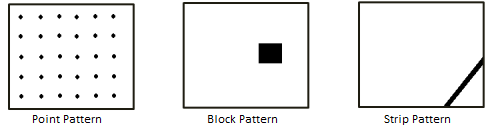
\includegraphics[width= 7cm,height=2cm]{ART_Patterns.png}
%\caption{Failure domains across input domain~\cite{chan1996proportional}}
%\label{fig:failurePatterns}
%\end{figure}
\begin{figure} [H]
\centering
\subfigure[Point domain]{
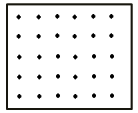
\includegraphics[width=2.5cm,height=2cm]{point.png}
\label{fig:point}
}
\subfigure[Block domain]{
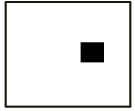
\includegraphics[width=2.5cm,height=2cm]{block.png}
\label{fig:block}
}
\subfigure[Strip domain]{
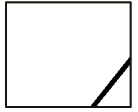
\includegraphics[width=2.5cm,height=2cm]{strip.png}
\label{fig:strip}
}

\caption{Failure domains across input domain~\cite{chan1996proportional}}
\label{fig:patterns2}
\end{figure}
%In Section~\ref{sec:adfd+} we describe the ADFD+ framework that can find the failure, its domain and plot the domain up to the specified range in a graphical form. Experiments confirms the successful working of ADFD+.


 

%%%%%%%%%%%%%%%%%    ADFD+   %%%%%%%%%%%%%%%%%%%

\section{Automated Discovery of Failure Domain+}\label{sec:adfd+}
ADFD+ is an improved and extended form of ADFD strategy developed previously by Ahmad and Oriol~\cite{ahmad2013adfd}. It is an automated framework which finds the failures and their domains within a specified range and present them on a graphical chart. 

The main improvements of ADFD+ over ADFD strategy are stated as follows.
\begin{itemize}
\item ADFD+ generates a single Java file dynamically at run time to plot the failure domains as compared to one Java file per failure in ADFD. This saves sufficient time and makes the execution process quicker.

\item ADFD+ uses (x, y) vector series to represent failure domains as opposed to the (x, y) line series in ADFD. The vector series allows more flexibility and clarity to represent a failure and its domain.   

\item ADFD+ takes a single value as range with in which the strategy search for a failure domain whereas ADFD takes two values for lower and upper bound representing x and y-axis respectively.

\item In ADFD+, the algorithm of dynamically generating Java file, created at run-time after a failure is detected, is made more simplified and efficient.

\item In ADFD+, the failure domain is focused in the graph, which gives a clear view of, pass and fail points. The points are also labelled for clarification as shown in Figure~\ref{fig:Workflow}. 

%The difference in representation of fault by ADFD and ADFD+ can be seen in figure .... Figure x is generated by ADFD with lower bound as ... and upper bound as ... While Figure Y is generated by ADFD+ with range ... for the same program given in appendix a. 
\end{itemize}


%%%%%%%%%%%%%%%%%%%%

\subsection{Workflow of ADFD+}
ADFD+ is a completely automatic process and all the user has to do is to specify the program to test and click the $Draw Fault Domain$ button. The default value for range is set to 5, which means that ADFD+ will search 83 values around the failure. On clicking the button YETI is executed with ADFD+ strategy to search for a failure in two-dimensional program. On finding a failure the ADFD+ strategy creates a Java file which contains calls to the program on the failing value and its surrounding values within the specified range. The Java file is compiled and executed and the result is analysed to check for pass and fail values. Pass and fail values are stored in pass and fail text files respectively. At the end of test, all the values are plotted on the graph with pass values in blue and fail values in red colour as shown in Figure~\ref{fig:adfdPlusExample}.
\\

%Instead of front end give workflow. It will make more sense. Change the code of the program

\begin{figure}[ht]
\centering
\includegraphics[width= 8.5cm,height=7cm]{adfdPlusWorkflow.png}
\caption{Workflow of ADFD+}
\label{fig:Workflow}
\end{figure}


%%%%%%%%%%%%%%%%%%%%
%ADFD+ is an extension of ADFD's algorithm with more accuracy to find and clarity to plot the failure domain on a graphical chart. Deriving failure domains using ADFD+ is a one click process and all the tester needs to input is the class to test and the range-value for which to search around the found failure. 
%%%%%%%%%%%%%%%%%%%%

\subsection{Implementation of ADFD+} \label{implementation_yeti}
The ADFD+ technique is implemented in YETI. The tool YETI is available in open-source at \url{http://code.google.com/p/yeti-test/}. A brief overview of YETI is given with the focus on parts relevant to implementation of ADFD+ strategy. YETI is a testing tool developed in Java that tests programs using random strategies in an automated fashion. YETI meta-model is language-agnostic which enables it to test 
programs written in functional, procedural and object-oriented languages. 

YETI consists of three main parts including core infrastructure for extendibility, strategies section for adjustment of multiple strategies and 
languages section for supporting multiple languages. Both strategies and languages sections have pluggable architecture to easily incorporate new strategies and 
languages making YETI a favourable choice to implement ADFD+ strategy. YETI is also capable of generating test cases to reproduce the failures found during the test session. 
The strategies section in YETI contains all the strategies including random, random+ and DSSR to be selected for testing according to the specific needs. The default test 
strategy for testing is random. In strategies package, on top of the hierarchy, is an abstract class $YetiStrategy$, which is extended by $YetiRandomPlusStrategy$ and is further extended to get ADFD+ strategy.

\begin{figure*}[ht]
\centering
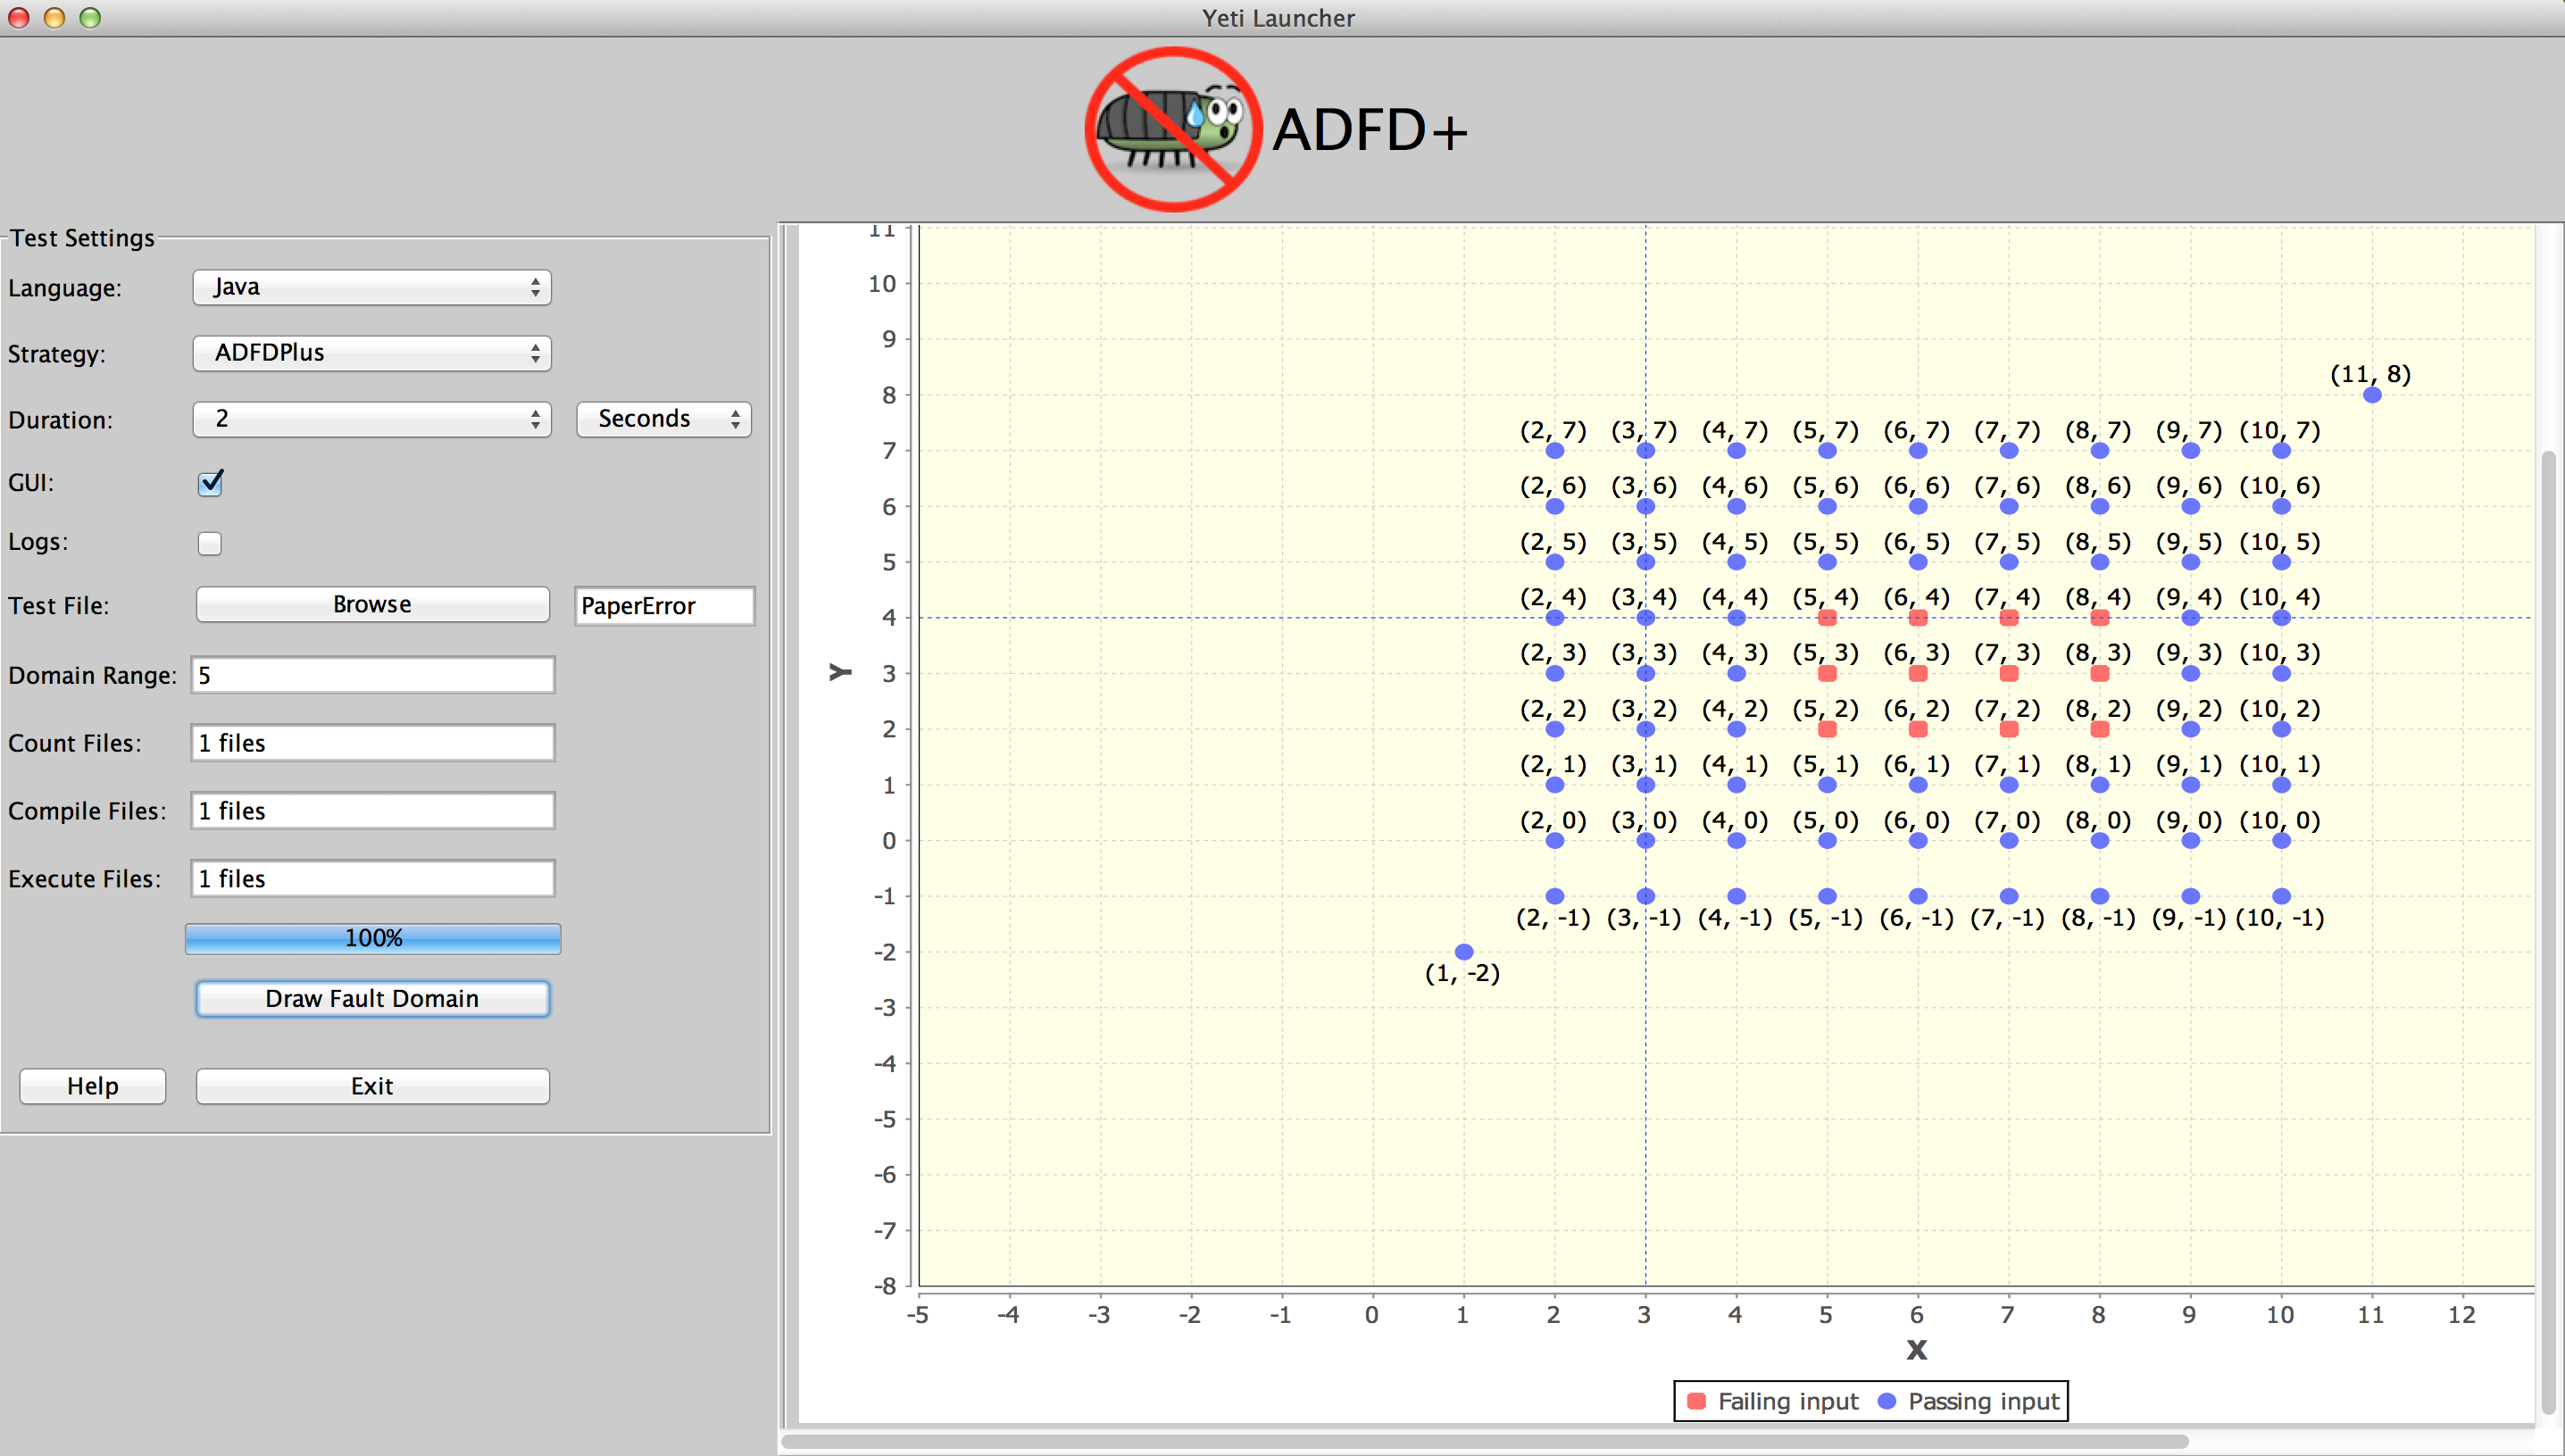
\includegraphics[width=17cm,height=10.2cm]{exampleError.png}
\caption{The output of ADFD+ for the above code.}
\label{fig:adfdPlusExample}
\end{figure*}

\subsection{Example to illustrate working of ADFD+}
Suppose we have the following error-seeded class under test. From the program code, it can be easily noticed that an $ArithmeticException$ (DivisonByZero) failure is generated when the value of variable $x$ ranges between 5 to 8 and the value of variable $y$ between 2 to 4.

\begin{lstlisting}
public class Error {
  public static void Error (int x, int y){
    int z;
    if (((x>=5)&&(x<=8))&&((y>=2)&&(y<=4)))
		 {
			 z = 50/0;
		 }
   } 
}
\end{lstlisting}
On test execution, the ADFD+ strategy evaluates the class with the help of YETI and finds the first failure at x = 6 and y = 3. Once a failure is identified ADFD+ uses the surrounding values around it to find a failure domain. The range of surrounding values is limited to the value set by the user in the $Domain Range$ variable. When the value of $Domain Range$ is 5, ADFD+ evaluates total of 83 values of $x$ and $y$ around the found failure. All evaluated (x, y) values are plotted on a two-dimensional graph with red filled circles indicating fail values and blue filled circles indicating pass values. Figure~\ref{fig:adfdPlusExample} shows that the failure domain forms a block pattern and the boundaries of the failure are $(5, 2), (5, 3),(5, 4), (6, 2), (6, 4), (7, 2), (7, 4), (8, 2), (8, 3), (8, 4)$. 





%%%%%%%%%%%%%%%%%%%%%%%%%%%%%%%%%%%%%%%%%%%%%%%%%

\section{Randoop}
Random tester for object oriented programs (Randoop) is a fully automatic tool, capable of testing Java classes and .Net binaries. It takes a set of classes to test, time limit or number of tests to stop and and optionally a set of configuration files to assist testing as input. Randoop checks for are assertion violations, access violations and un-expected program termination in a given class. Its output a suite of JUnit for Java and NUnit for .Net program. Each unit test in a test suite is a sequence of method calls (hereafter referred as sequence). Randoop builds the sequence incrementally by randomly selecting a public method from the class under test and arguments for these methods are selected from the pre-defined pool in case of primitive types and as sequence of null values in case of reference type. It uses feedback mechanism to filter out duplicate test cases. 

 


%Randoop maintains two sets called \verb+ErrorSeqs+ and \verb+NonErrorSeqs+ to record the feedback. It extends \verb+ErrorSeqs+ set in case of contract or filter violation and \verb+NonErrorSeqs+ set when no violation is recorded in the feedback. The use of this dynamic feedback evaluation at runtime brings an object to an interesting state. On test completion, \verb+ErrorSeqs+ and \verb+NonErrorSeqs+ are produced as JUnit/NUnit test suite. In terms of coverage and number of faults discovered, Randoop implementing FDRT was compared with JCrasher and JavaPathFinder and 14 libraries of both Java and .Net were evaluated~\cite{visser2004test}. The results showed that Randoop achieved more branch coverage and better fault detection than JCrasher. 



%Daikon is a tool~\cite{ernst2007daikon}, which uses machine-learning technique to automatically generate likely invariants of the program written in C, C++, Java and Pearl. Daikon takes the program and a few test cases as input. The test cases may be either generated manually or by an automated tool. Daikon executes the test cases on the program under test and observes the values that the program computes. At the end of the test session it reports the properties that were true for the observed executions. A feature of Daikon facilitate to process the generated invariants to mitigate non-interesting and redundant invariants. Another feature allows to inserts the generated invariants in to the source code as assertions. The report generated by Daikon is useful in understanding program logic, generating invariants, predicting incompatibilities in component integration, automating theorem proving, repairing inconsistencies in data structures and checking the validity of data streams.




%%%%%%%%%%%%%%%%%    EVALUATION   %%%%%%%%%%%%%%%%%%%%
%\section{Comparison of ADFD+ \& Randoop}\label{sec:eval}
%In order to check the performance and efficiency of ADFD+ we compared it with a random testing tool Randoop. Our subject classes for these experiments were the same that were used in evaluation of ADFD \cite{ahmad2013adfd}. We ran ADFD+ and Randoop for 30 times on each error-seeded one and two dimensional numerical programs, measuring its effectiveness by the total number of test cases used to detect all the failures and its efficiency by the CPU time consumed. 

\section{Research questions}
Beside the main question of finding the performance of ADFD+ with respect to time and number of test cases, the following research questions have also been addressed in this study:
\begin{enumerate}
\item \textbf{Efficiency:} How efficient is ADFD+, compared to Randoop, across different input domains?
\item \textbf{Effectiveness:} How effective is ADFD+, compared to Randoop, across different input domains?
\item \textbf{Failure-domains:} How the boundaries of a failure domains are presented by ADFD+ and Randoop?
%5 you will also prove it through figure but you can also say ADFD+ clarify it further by showing the boundaries in graphical form.
\end{enumerate}


%Because of using error-seeded one and two dimensional numerical programs, we were aware of the failure domain present in each program. The correct identification and presentation of the failure domain by ADFD+ prove the correct working of ADFD+. We then evaluated the same program by Randoop. 


\begin{figure*}[!Htp]
\centering
\begin{minipage}{.5\textwidth}
  \centering
  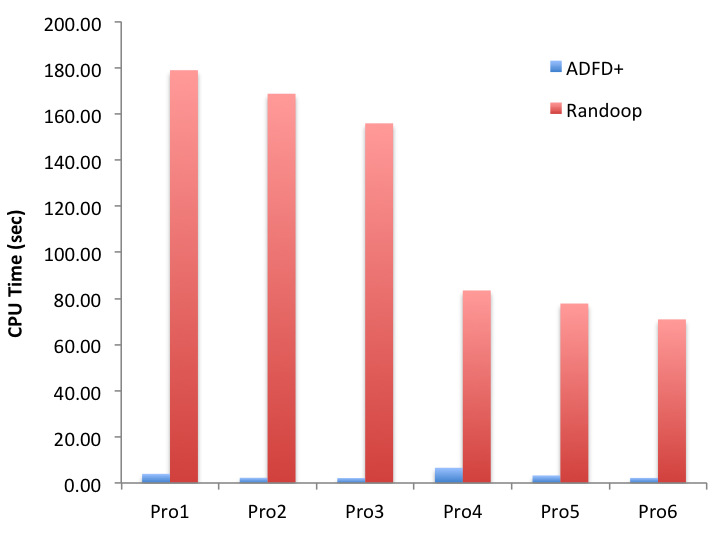
\includegraphics[width=7.5cm,height=8cm]{timeTakenBar.png}
  \caption{Time taken to find failure domains}
  \label{fig:testtime}
\end{minipage}%
\begin{minipage}{.5\textwidth}
  \centering
  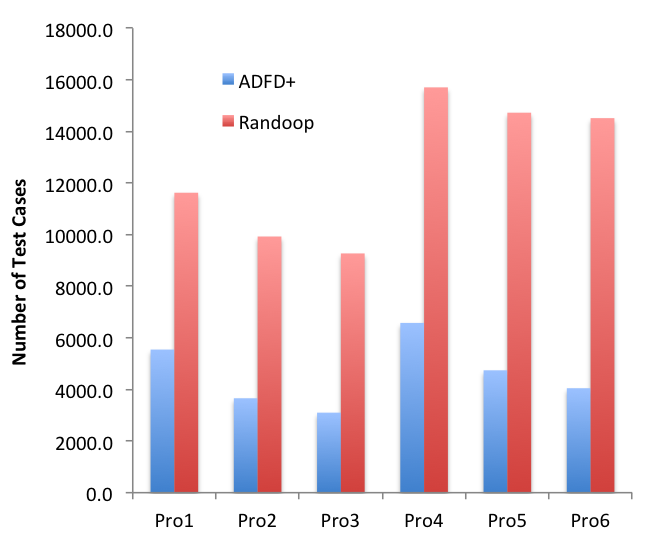
\includegraphics[width=7.5cm,height=8cm]{testCasesBar.png}
  \caption{Test cases taken to find failure domains}
  \label{fig:testcases}
\end{minipage}
\end{figure*}

\section{Evaluation} \label{evaluation}
To evaluate the performance and efficiency of ADFD+, we followed the common practice \cite{oriat2005jartege, pacheco2005eclat, xie2005symstra} which is to compare it against another random testing tool. We used Randoop for comparison. We carried out testing of several error-seeded one and two dimensional numerical programs written in Java. Our subject programs were the same used in evaluation of ADFD \cite{ahmad2013adfd}. The programs were divided in to two sets. Set A and B contains one and two-dimensional programs respectively. Each class was injected with at least one failure domain of point, block or strip nature. The values forming the failure domains are given in Table \ref{table:failureDomains}. Every program was tested independently for 30 times by both ADFD+ and Randoop on the basis of time taken and number of tests used to find all the failures. The external parameters were kept constant in each test. Due to the absence of contracts and assertions in the code under test, undeclared exceptions were taken as failures in accordance with the previous studies~\cite{ahmad2013adfd, Oriol2012}.

%The code for the programs under test is given in Appendix~\ref{} while the test details are presented in Table~\ref{table:Results}. 
%Every class was evaluated through $10^5$ calls in each test session of ADFD+.
%\footnote{The total number of tests is equal to $60\times 30\times 3 \times 10^5 = 540\times10^6~tests$.} 
\subsection{Experimental setup}
All experiments were conducted with a 64-bit Mac OS X Mountain lion version 10.8.5 running on 2.7 GHz Intel Core i7 with 16 GB (1600 MHz DDR3) of RAM. YETI runs on top of the Java\texttrademark  SE Runtime Environment [version 1.6.0\_35]. %The machine took approximately 100 hours to process the experiments.
The ADFD+ Jar file is available at \url{https://code.google.com/p/yeti-test/downloads/list/} and Randoop at \url{https://randoop.googlecode.com/files/randoop.1.3.3.zip}.

The following commands (1) and (2) were used to run the ADFD+ and Randoop. Both ADFD+ and Randoop were executed with default settings except that Randoop was provided with a seed value.% On running command (1) the ADFD+ starts with a GUI front-end given in Figure \ref{fig:adfdPlusExample}. On running command (2) Randoop starts in CLI mode as there is no GUI.
\begin{lstlisting}[language=bash]
$ java -jar adfd_yeti.jar -------------(1)

$ java randoop.main.Main gentests \
--testclass=OneDimPointFailDomain \
--testclass=Values --timelimit=100 ----(2)
\end{lstlisting}



%\begin{table}[h]
%\caption{Table depicting values of x and y arguments forming point, block and strip failure domain in Figure 6(a), 6(b), 6(c) and Figure 7(a), 7(b), 7(c) respectively}
%\centering
%{\renewcommand{\arraystretch}{1.1}
%\begin{tabular}{|l|l|l|l|}
%\hline
%Dim & Point failure		& 	Block failure		& 	Strip failure		\\
%\hline
%One & x = -66			&	x = -1, 0, 1		&	x = -4 -- 34 	\\	
%& x = -2			 	&	x =-26 -- -29	&					\\	
%& x= 51 				&	x = 51 -- 54 	&					\\
%& x= 23 				& 	 				& 					\\
%\hline
%Two &x=2, y=10			&	x = 5, y = 2		&	x = 7,~~y = 0	\\	
%&x=4, y=10			&	x = 6, y = 2		&	x = 8,~~y = 0	\\	
%&x=7, y=10			&	x = 7, y = 2		&	x = 8,~~y = 1	\\
%&x=9, y=10			& 	x = 8, y = 2 		& 	x = 9,~~y = 1	\\
%&					& 	x = 5, y = 3 		& 	x = 9,~~y = 2	\\
%&					& 	x = 6, y = 3 		& 	x = 10, y = 2	\\
%&					& 	x = 7, y = 3 		& 	x = 10, y = 3	\\
%&					& 	x = 8, y = 3 		& 	x = 11, y = 3	\\
%&					& 	x = 5, y = 4 		& 	x = 11, y = 4	\\
%&					& 	x = 6, y = 4 		& 	x = 12, y = 4	\\
%&					& 	x = 7, y = 4 		& 	x = 12, y = 5	\\
%&					& 	x = 8, y = 4 		& 	x = 13, y = 6	\\
%&					&			      		& 	x = 14, y = 6	\\				
%&					&			      		& 	x = 14, y = 7	\\
%\hline
%\end{tabular}
%}
%\bigskip
%\label{table:failureDomains}
%\end{table}


\section{Experimental results}
%The experimental results show that the ADFD+ outperformed Randoop in both the time taken and number of tests used to detect all the injected faults. The ADFD+ also provide the added benefit of presenting the results in graphical form as shown in Figure \ref{fig:failureDomainsOneDimension} and \ref{fig:failureDomainsTwoDimension}. 
Results are split in to two sections depicting efficiency and effectiveness of the two tools.
\subsection{Efficiency Evaluation}
Figure \ref{fig:testtime} shows the efficiency measurement of the ADFD+ and Randoop against the selected programs. The x-axis represents one and two-dimensional programs with point, block and strip failure domain. The y-axis represents average time taken by both the tools to detect the whole failure domains. ADFD+ outperformed Randoop in the time taken to discover all forms of failure domains. Overall, this answers \textbf{RQ1} positively. The experimental analysis shows that there is a sufficient gain in efficiency when ADFD+ is used. The amount of gain in efficiency is up to two orders of magnitude.

It should be noted that the part of the gain may also be due to the fast processing of the underlying tool YETI, which is capable of executing $10^6$ test calls per minute on Java code. Therefore, to find the performance of only ADFD+ we performed the second set of experiments to measure effectiveness.

%For finding the efficiency, the CPU time consumed from the start of the test to the identification of last failure was measured for each experiment of ADFD+ and Randoop.  Figure \ref{fig:testtime} shows the results in a box-and-whisker plot. The figure shows that ADFD+ in no case took more than ten seconds to find the failures where Randoop consumed at least  80 seconds to find the same failures.
\subsection{Effectiveness Evaluation}
Figure \ref{fig:testcases} shows the effectiveness measurement by ADFD+ and Randoop to find the whole failure domains. The x-axis represents one and two-dimensional programs with point, block and strip failure domain. The y-axis represents average number of test cases used by both the tools to detect the whole failure domains. The ADFD+ uses sufficiently lower number of test cases as compared to Randoop to find the whole failure domains. The amount of gain in performance is up to 50\% or more. This provide a positive answer for \textbf{RQ2}.

\subsection{Failure Domains}
Both the tools found all the failure domains in specific time or using specific number of test cases. The ADFD+ also provide the added benefit of presenting the failure domains in graphical form as shown in Figure \ref{fig:failureDomainsOneDimension} and \ref{fig:failureDomainsTwoDimension}. The red and blue circle represents the failing and passing values respectively. The user can also enable or disable the option of showing the failing values on the graph. In Randoop there is no graphical representation or textual option to show failure domains separately. This provide a positive answer for \textbf{RQ3}.


%\subsubsection{Test of one-dimension programs by ADFD+}
%In each of the 30 experiments, The ADFD+ successfully discovered and plotted the failure domains for point, block and strip pattern as shown in the Figure~\ref{fig:failureDomainsOneDimension}. The lower and upper bound for each experiment are set to -100 and 100 respectively.

%\subsubsection{Test of two-dimension programs by ADFD+}
%In each of the 30 experiments, The ADFD+ once again successfully discovered and plotted the failure domain for point, block and strip failure domain as shown in the Figure~\ref{fig:failureDomainsTwoDimension}. The range value for each experiment is set to 10. Labels are disabled in the charts given in Figure~\ref{fig:failureDomainsTwoDimension} for clarity purpose. The failure values in each of the point, block and strip failure domain is given in Table~\ref{table:failureDomains}. 

%\subsection{Daikon results} \label{daikon_results}
%In initial set of experiments, Daikon failed to generate an invariant for identifying a single failure. On analysis It is found that Daikon rely on the existing set of test cases to generate invariants. Since the test cases produced by Randoop did not generate any test case from failure domain therefore Daikon could not generate an assertion to point out the failure. To enable Randoop to generate test case from failure domain we directed it to produce random values between a limited range. In this way we were able to generate interesting test cases from Randoop. Test results of Randoop are shown in Table \ref{}

%\begin{figure}[!Htp]
%\centering
%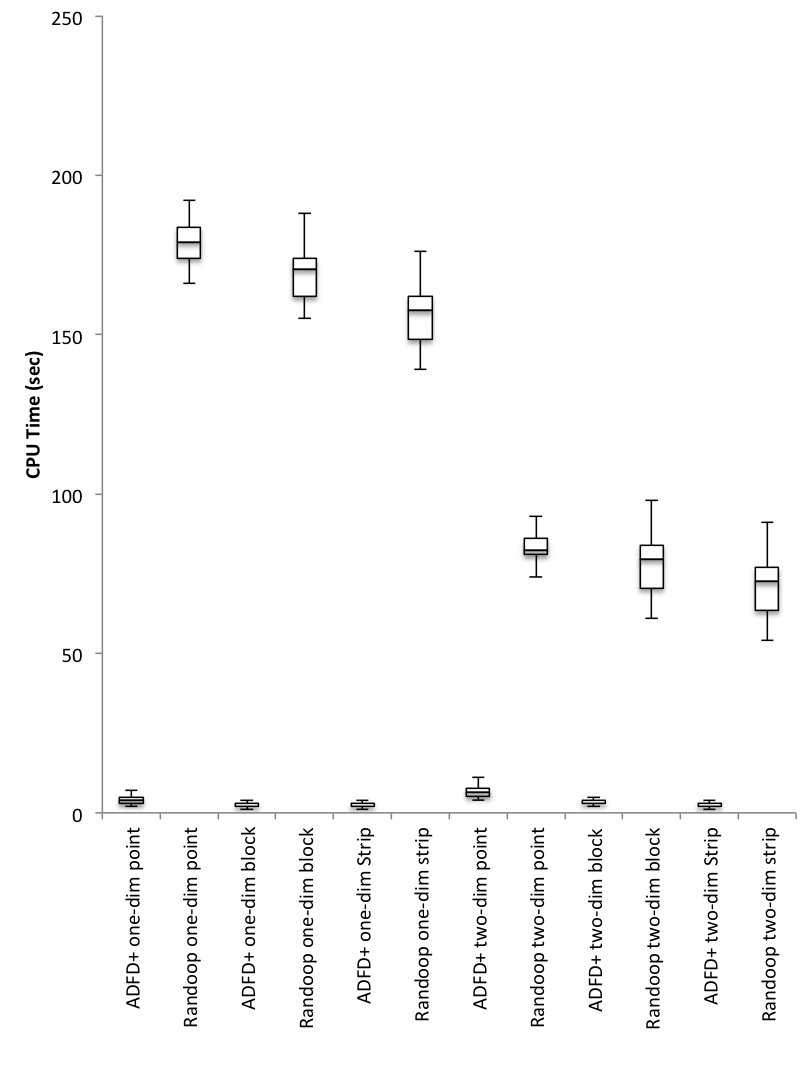
\includegraphics[width=8.7cm,height=6.5cm]{timetaken.png}
%\caption{Time taken to find failures}
%\label{fig:timelimit}
%\end{figure}

%\begin{figure}[!Htp]
%\centering
%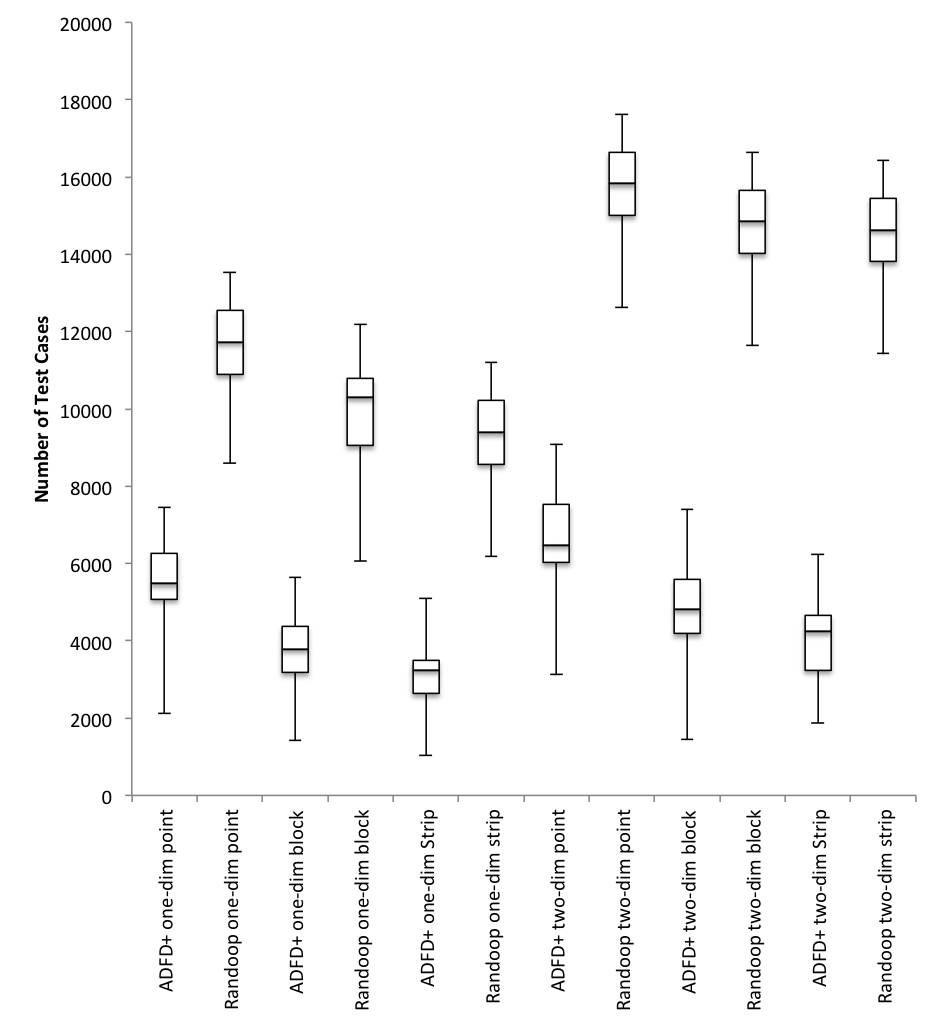
\includegraphics[width=8.7cm,height=6.5cm]{TestCases.png}
%\caption{Number of test cases taken to find failures}
%\label{fig:numberoftests}
%\end{figure}










%\begin{table*}[htp]
%\caption{Randoop Results}
%\centering
%{\renewcommand{\arraystretch}{1.2}
%\begin{tabular}{|l|l|r|r|r|r|r|}
%\hline
%Program	 dimension	& 	Failure domain	& 	Test time 	& Random range	& Total TC & Pass TC		& Fail TC		%\\
%\hline
%One					&	Point			&	60 sec		& -100 to 100	& 82	    & 79			& 3				%\\
%One					&	Block			&	60 sec		& -100 to 100	& 82	    & 75			& 7				%\\
%One					&	Strip			&	60 sec		& -100 to 100	& 82	    & 62			& 22			%	\\
%Two					&	Point			&	60 sec		& -100 to 100	& 6563	    & 6521		& 42			%	\\
%Two					&	Block			&	60 sec		& -100 to 100	& 5902	    & 5057		& 845			%	\\
%Two					&	Strip			&	60 sec		& -100 to 100	& 6226	    & 3896		& 2330			%	\\
%\hline
%\end{tabular}
%}
%\bigskip
%\label{table:failureDomains}
%\end{table*}


%\subsubsection{Test of one-dimensional programs by Daikon}




%\subsubsection{Test of two-dimensional programs by Daikon}





%\begin{table*}[ht]
%\caption{Table depicting values of failure points identified by ADFD+ Daikon}
%\centering
%{\renewcommand{\arraystretch}{1.3}
%\begin{tabular}{|l|l|r|r|r|r|}
%\hline
%Technique 	& Dimension	& Test cases		& 	Point failure		& 	Block failure	& 	Strip failure	\\
%\hline
%ADFD+		& 	One				& N/A			& 					& 				&				\\
%Daikon		& 	One				& 10			&					&				&				\\
%Daikon		& 	One				& 20			&					&				&				\\
%ADFD+		& 	Two				& N/A			&					&				&				\\
%Daikon		& 	Two				& 10			&					&				&				\\
%Daikon		& 	Two				& 20			&					&				&				\\
%\hline
%\end{tabular}
%}
%\bigskip
%\label{table:results}
%\end{table*}




%for point, block and strip of one dimensional program. Use the same programs of ADFD, same figures but analyse it again on Daikon. because ADFD and ADFD+ behave in the same way for one dimension. For point block and strip of two dimensional programs. Use adfd+ system.






\section{Discussion}
We have shown that ADFD+ is a promising technique to find a failure and using it as a focal point find the whole failure domain. We have also shown that ADFD+ can graphically draw the failure domain on a chart. The pictorial representation of failure domain helps in easily identifying the underlying domain and its boundaries, which can be helpful to developers in debugging.

As a pilot study, we also ran an empirical study to evaluate several error-seeded programs. While it would be surprising if production programs produced much different results, it would be worthwhile to check.

More importantly, the implementation of ADFD+ for this pilot study has significant limitations in practice, as it requires only one and two dimensional numerical programs. Though it is not difficult to extend the approach to test more than two-dimensional programs containing other primitive types, it would however be difficult to plot them on the chart as the number of coordinates increases. The approach can also be extended to test object-oriented programs by implementing objects distance proposed by Ciupa et al. \cite{ciupa2006object}. The details of such an implementation will take some effort.

The ADFD+ range value specifies how many values to test around the failure. The range can be set to any number before the test starts. The value of range is directly proportional to the time taken because the higher the range value the higher number of values to test. Higher range value also leads to a very large graph and the tester has to use the zoom feature of graph to magnify the failure region.




\section{Threats to validity}
The research study faces threats to external and internal validity. The threats to external validity are the same, which are common to most of the empirical evaluations i.e. to what degree the classes under test and test generation tool (Randoop) are representatives of true practice. The classes under test contains failure patterns in only one and two-dimensional input domain. The threats may be reduced to a greater extent in future experiments by taking several types of classes and different test generation tools. 

The threat to internal validity includes annotation of invariants that can bias the results, which may have been caused by error-seeded classes used in our experiments. Internal threats may be avoided by taking real classes and failures in the experiments. Moreover, testing a higher number of classes will also increase the validity of the results.

\section{Conclusion}
Automated Discovery of Failure Domain+ (ADFD+) is distinctive from other random test strategies in the sense that it is not only limited to identifying a failure in the program. Instead, the failure is exploited to identify and graphically plot its failure domain.

In the first section, we describe ADFD+ in detail which is based on our previous approach ADFD~\cite{ahmad2013adfd}. We then describe the main improvements of ADFD+ over ADFD. 

In the second section, we analysed and compared the results of the experiments performed by both ADFD+ and Daikon in the case of programs with point, block and strip failure domain. 

We showed that Daikon lakes to accurately identify the failure boundary and therefore cannot generate invariants for such failures.  We further explain why Daikon does not work well for boundary failures. The main reason we identified for this behaviour is Daikons dependence on initial set of test cases, which are required by Daikon for generating invariants. With increase in number of test suite or high quality test suite improves the performance of invariants. 

\section{Future Work} \label{futurework}
The current approach can be extended to a larger set of real world multi-dimensional programs, using real failure instead of error-seeded programs. However, to plot failure domains of complex multi-dimensional nature, more sophisticated graphical tools like Matlab will be required rather than JFreeChart used in the current study. This may not restrict the formation of new failure domains to point, block and strip failure domain in one and two-dimensional numerical programs. 


























%%%%%%%%%%%%%%%%%    ACKNOWDLEGEMENT   %%%%%%%%%%%%%%%%%%%%
\section{Acknowledgments}
% should put it back in final version
The authors thank the Department of Computer Science, University of York for its financial support with the Departmental Overseas Research Scholarship (DORS) award. We also thanks to Richard Page for his valuable help and generous support.




%
% The following two commands are all you need in the
% initial runs of your .tex file to
% produce the bibliography for the citations in your paper.
\bibliographystyle{abbrv}
\bibliography{sigproc}  % sigproc.bib is the name of the Bibliography in this case
% You must have a proper ".bib" file
%  and remember to run:
% latex bibtex latex latex
% to resolve all references
%
% ACM needs 'a single self-contained file'!
%
%APPENDICES are optional
%\balancecolumns
\bigskip


\begin{wrapfigure}{l}{0.12\textwidth}
  \vspace{-15pt}
  \begin{center}
    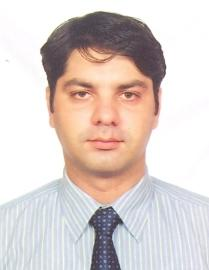
\includegraphics[width=0.13\textwidth]{mian.jpg}
    \bigskip
    \\
    \bigskip
      
\includegraphics[width=0.13\textwidth]{manuel.jpg}
  \end{center}
  \vspace{-20pt}
\end{wrapfigure}
\noindent\textbf{Mian Asbat Ahmad} is a PhD scholar at the Department of Computer Science, the University of York, UK. He completed his M(IT) and MS(CS) from Agric. University Peshawar, Pakistan in 2004 and 2009 respectively. His research interests include new automated random software testing strategies.


\bigskip
\noindent\textbf{Manuel Oriol} is a lecturer at the Department of Computer Science, the University of York, UK. He completed his PhD from University of Geneva and an MSc from ENSEEIHT in Toulouse, France. His research interests include software testing, software engineering, middleware, dynamic software updates, software architecture and real-time systems.



\newpage
Appendix 
\begin{figure} [H]
\subfigure[Point failure domain in one-dimension]{
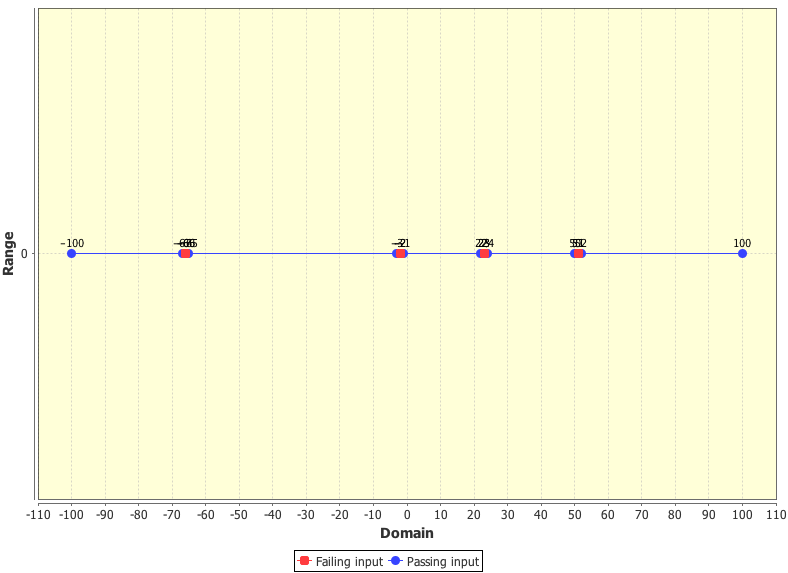
\includegraphics[width=8cm,height=6cm]{PFDOne.png}
\label{fig:PFDOne}
}
\subfigure[Block failure domain in one-dimension]{
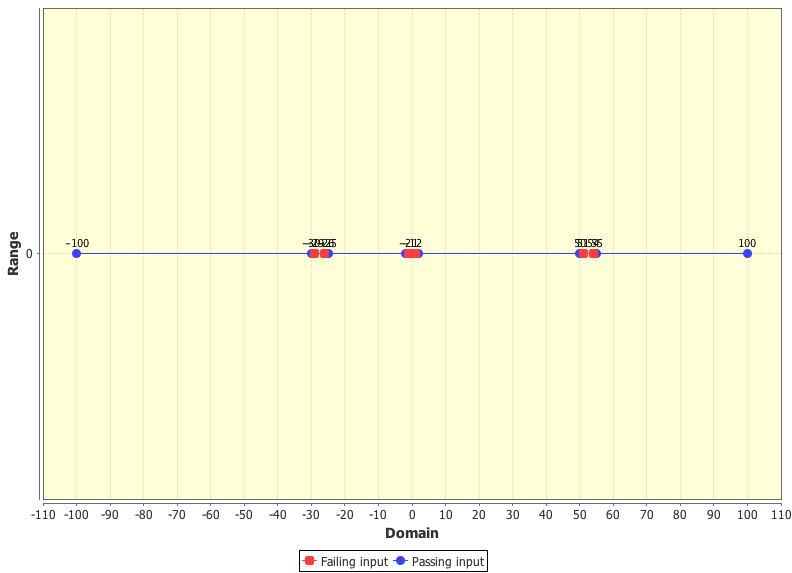
\includegraphics[width=8cm,height=6cm]{BFDOne.png}
\label{fig:BFDOne}
}
\subfigure[Strip failure domain in one dimension]{
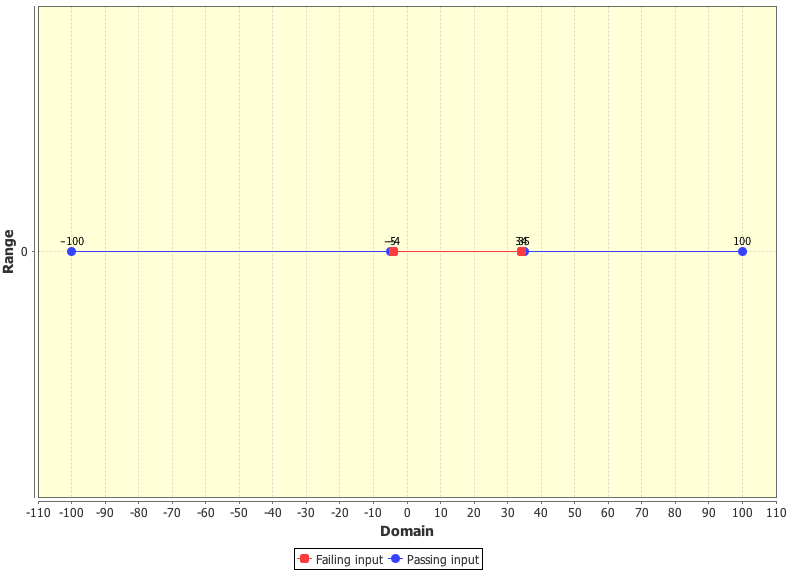
\includegraphics[width=8cm,height=6cm]{SFDOne.png}
\label{fig:SFDOne}
}
\caption{Pass and fail values of plotted by ADFD+ in three different cases of two-dimension programs}

\label{fig:failureDomainsOneDimension}
\end{figure}




\begin{figure} [H]

\subfigure[Point failure domain in two-dimension]{
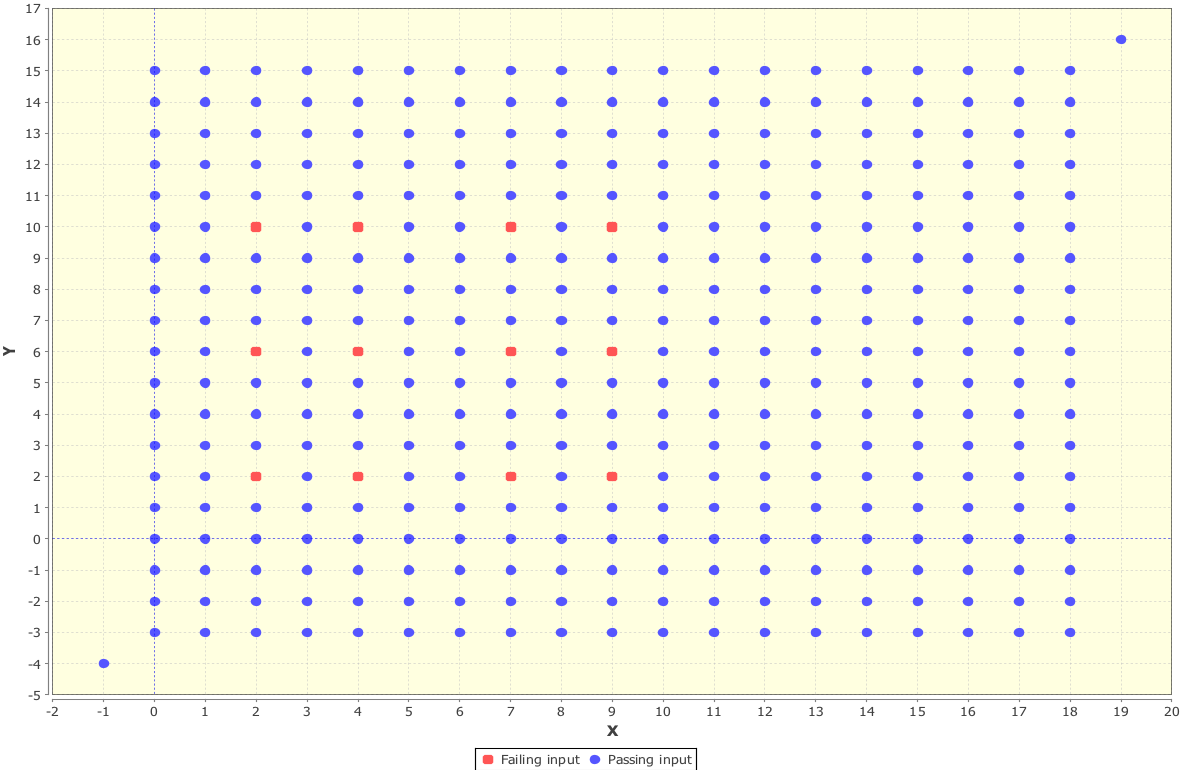
\includegraphics[width=8cm,height=6cm]{PFDTwo.png}
\label{fig:PFDOne}
}
\subfigure[Block failure domain in two-dimension]{
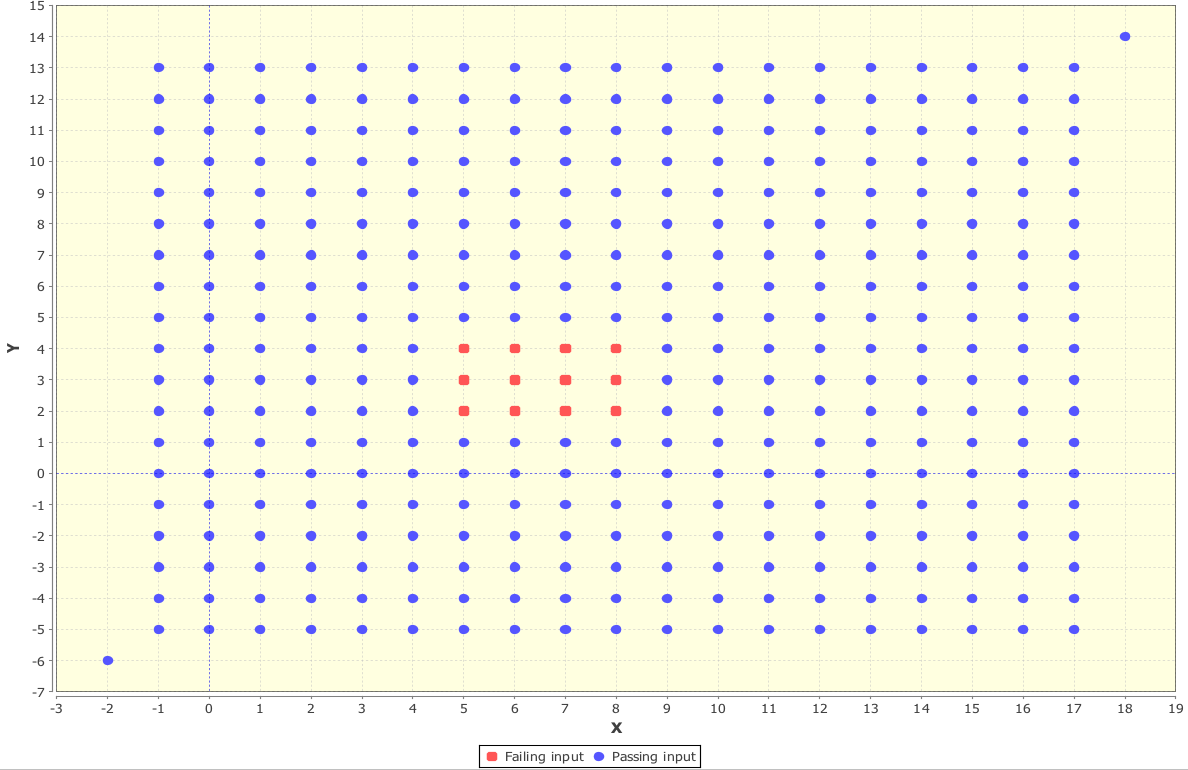
\includegraphics[width=8cm,height=6cm]{BFDTwo.png}
\label{fig:BFDOne}
}
\subfigure[Strip failure domain in two-dimension]{
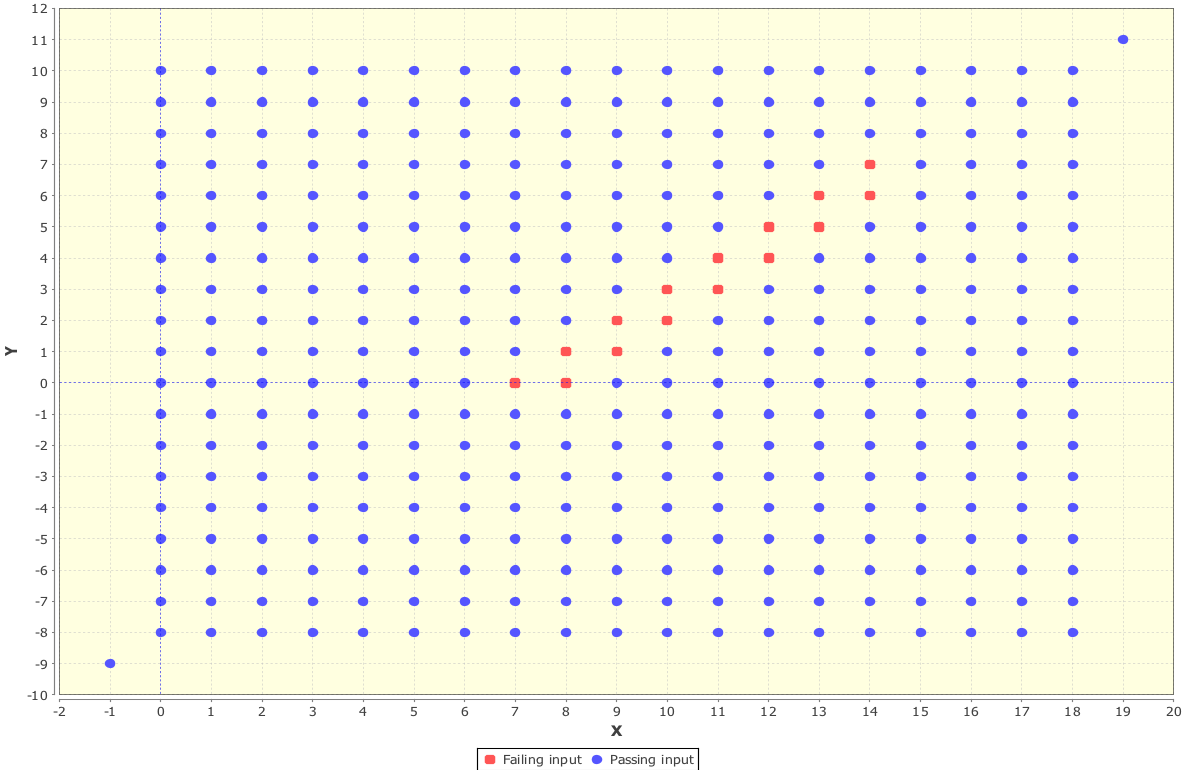
\includegraphics[width=8cm,height=6cm]{SFDTwo.png}
\label{fig:SFDOne}
}
\caption{Pass and fail values of plotted by ADFD+ in three different cases of two-dimension programs}

\label{fig:failureDomainsTwoDimension}
\end{figure}


































\begin{comment}

%%%%%%%%%%%%%%%%%%%%%%%%%%%%%%%%%%%%%%%%%%%%%%%%%%%%%%%%%%%%%%%%%%%%%%%%%%%%%%%%%%%%%%%%%%%%%%
\scriptsize
\textbf{Program 2} Point domain with One argument
\begin{lstlisting} 
/**
 * Point Fault Domain example for one argument
 * @author (Mian and Manuel)
 */
public class PointDomainOneArgument{

	public static void pointErrors (int x){
		if (x == -66 )
			x = 5/0;

		if (x == -2 )
			x = 5/0;

		if (x == 51 )
			x = 5/0;

		if (x == 23 )
			x = 5/0;
	}
}
\end{lstlisting}
%%%%%%%%%%%%%%%%%%%%%%%%%%%%%%%%%%%%%%%%%%%%%%%%%%%%%%%%%%%%%%%%%%%%%%%%%%%%%%%%%%%%%%%%%%%%%%
\textbf{Program 3} Point domain with two argument
\begin{lstlisting}
/**
 * Point Fault Domain example for two arguments
 * @author (Mian and Manuel)
 */
public class PointDomainTwoArgument{

	public static void pointErrors (int x, int y){
		int z = x/y;
	}

}
\end{lstlisting}

%%%%%%%%%%%%%%%%%%%%%%%%%%%%%%%%%%%%%%%%%%%%%%%%%%%%%%%%%%%%%%%%%%%%%%%%%%%%%%%%%%%%%%%%%%%%%%
\textbf{Program 4} Block domain with one argument
\begin{lstlisting}
/**
 * Block Fault Domain example for one arguments
 * @author (Mian and Manuel)
 */

public class BlockDomainOneArgument{

public static void blockErrors (int x){
	
	if((x > -2) && (x < 2))
		x = 5/0;
	
	if((x > -30) && (x < -25))
		x = 5/0;
	
	if((x > 50) && (x < 55))
		x = 5/0;

   }
}

\end{lstlisting}
%%%%%%%%%%%%%%%%%%%%%%%%%%%%%%%%%%%%%%%%%%%%%%%%%%%%%%%%%%%%%%%%%%%%%%%%%%%%%%%%%%%%%%%%%%%%%%
\textbf{Program 5} Block domain with two argument
\begin{lstlisting}
/**
 * Block Fault Domain example for two arguments
 * @author (Mian and Manuel)
 */
public class BlockDomainTwoArgument{

	public static void blockErrors (int x, int y){

		if(((x > 0)&&(x < 20)) || ((y > 0)&&(y < 20))){
		x = 5/0;
		}
  	
	}

}
\end{lstlisting}
%%%%%%%%%%%%%%%%%%%%%%%%%%%%%%%%%%%%%%%%%%%%%%%%%%%%%%%%%%%%%%%%%%%%%%%%%%%%%%%%%%%%%%%%%%%%%%

\textbf{Program 6} Strip domain with One argument
\begin{lstlisting}
/**
 * Strip Fault Domain example for one argument
 * @author (Mian and Manuel)
 */

public class StripDomainOneArgument{

	public static void stripErrors (int x){
	
		if((x > -5) && (x < 35))
			x = 5/0;
  	 }
}
\end{lstlisting}
%%%%%%%%%%%%%%%%%%%%%%%%%%%%%%%%%%%%%%%%%%%%%%%%%%%%%%%%%%%%%%%%%%%%%%%%%%%%%%%%%%%%%%%%%%%%%%
\textbf{Program 7} Strip domain with two argument
\begin{lstlisting}
/**
 * Strip Fault Domain example for two arguments
 * @author (Mian and Manuel)
 */
public class StripDomainTwoArgument{

	public static void stripErrors (int x, int y){

		if(((x > 0)&&(x < 40)) || ((y > 0) && (y < 40))){
		x = 5/0;
		}
  	
	}

}

\end{lstlisting}
%%%%%%%%%%%%%%%%%%%%%%%%%%%%%%%%%%%%%%%%%%%%%%%%%%%%%%%%%%%%%%%%%%%%%%%%%%%%%%%%%%%%%%%%%%%%%%

\end{comment}
\end{document}
